\documentclass[../talk.tex]{subfiles}
\begin{document}

\begin{frame}{Automata theory}
    \begin{overlayarea}{\slidewidth}{\slideheight}

        \begin{center}

            \vspace*{3em}

            \alert{The automata-theoretic approach to verification}

            \vspace*{2em}

            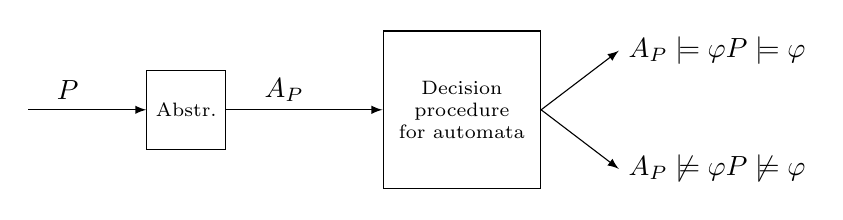
\begin{tikzpicture}
                \node (origin) [coordinate] at (0.5,0) {};

                \node (abstr) at (2,0) [minimum width=1cm, minimum height=1cm, anchor=west,draw] {};

                \node (rect) at (5,0) [minimum width=2cm,minimum height=2cm, anchor=west,draw] {};

                \node (yes) [coordinate] at (8,0.75) {};
                \node (no) [coordinate] at (8,-0.75) {};
                \path [->,>=latex]
                    (origin) edge (abstr.west)
                    (abstr.east) edge (rect.west)
                    (rect.east) edge (yes)
                    (rect.east) edge (no)
                ;

                \node at (1,0.25) {$P$};

                \node at (3.75,0.25) {$A_P$};

                \node [right of=yes, node distance=0cm, anchor=west] {$A_P \models \varphi \alert{\implies P \models \varphi}$};
                \node [right of=no, node distance=0cm, anchor=west] {$A_P \not\models \varphi \alert{\implies P \not\models \varphi}$};

                \node [align=center, text width=1cm, font=\scriptsize] at (abstr) {Abstr.};
                \node [align=center, text width=2cm, font=\scriptsize] at (rect) {Decision procedure for automata};
            \end{tikzpicture}
        \end{center}

    \end{overlayarea}
\end{frame}

\end{document}
